\documentclass[a4paper,english,12pt]{article}
%\usepackage[lwarpmk]{lwarp}
\usepackage{titlesec}
\usepackage{cc}
\usepackage{amsmath}
\usepackage[T1]{fontenc}
\usepackage[usenames,dvipsnames]{color}
\graphicspath{ {./images/} }
\usepackage[dvipsnames]{xcolor}
\titleformat*{\section}{\color{Brown}\normalfont\bfseries\Large}
\usepackage{prettyref}
\usepackage{amsthm}
\usepackage{amsmath}
\usepackage{amssymb}
\usepackage{float}
\usepackage{natbib}
\bibliographystyle{unsrtnat}
\PassOptionsToPackage{normalem}{ulem}
\usepackage{ulem}
\usepackage{mathptmx}
\usepackage{framed}
\usepackage{array}
\usepackage{csvsimple,longtable,booktabs}
\newlength{\mycolwidth}
\settowidth{\mycolwidth}{2cm} % widest entry


%\usepackage[unicode=true,pdfusetitle,
% bookmarks=true,bookmarksnumbered=false,bookmarksopen=false,
% breaklinks=false,pdfborder={0 0 1},backref=section,colorlinks=false]{hyperref}

\usepackage{pdfcomment}

%\newcommand{\dania}[1]{}
%\newcommand{\joyce}[1]{}
\newcommand{\chenc}[1]{\pdfcomment[author=Chen,color={1 0.5 0.5},subject={#1}]{#1}}
\newcommand{\dania}[1]{\pdfcomment[author=Dania,color={1 1 1},subject={#1}]{#1}}
\newcommand{\joyce}[1]{\pdfcomment[author=Joyce,color={1 0 1},subject={#1}]{#1}}
%\geometry{bindingoffset=2cm}


\usepackage{lipsum}

\hypersetup{colorlinks,
	linkcolor=red!95!black,%YellowOrange!85!black,
	citecolor=blue!85!black,
	pagecolor=blue!95!black,%
        urlcolor=magenta,filecolor=magenta,breaklinks,%
        dvips,bookmarks,bookmarksopen}

%\hypersetup{
%  linkcolor  = violet!\myshade!black,
%  citecolor  = YellowOrange!\myshade!black,
%  urlcolor   = Aquamarine!\myshade!black,
%  colorlinks = true
%}

\makeatletter
%\usepackage{pgfplots}
%\usepackage{tikz}
%\usepgfplotslibrary{external}
%\usetikzlibrary{external}
%\usepgflibrary{ plotmarks }
%\usetikzlibrary{arrows}
%\usetikzlibrary{plotmarks}
%\tikzexternalize[prefix = resource/]%, mode=list and make
%\tikzset{external/mode=graphics if exists}
%% the following forces redraw of all, if you reorder graphs
%tikzset{external/force remake}
\usepackage{microtype}
%
\usepackage{doi}
%\bibpunct{(}{)}{;}{a}{,}{,}

\renewcommand{\MakeUppercase}[1]{\color{green!50!black}\textsf{#1}}
%\usepackage{pdfsync}
\usepackage{amsfonts}
\usepackage{amscd}
\usepackage{bm}
\usepackage{euler}
\usepackage{url}
%\graphicspath{resource/}
%\graphicspath{./resource/}
\newcommand{\pde}{{\textsc{pde}}}
\newcommand{\res}{{\operatorname{Res}}}
\newcommand{\D}[2]{\frac{\partial #1}{\partial #2}}
\newcommand{\DD}[2]{\frac{\partial^2 #1}{\partial #2^2}}
\newcommand{\pp}{{}+}
\newcommand{\Ord}{\mathcal{O}}
\newcommand{\LL}{\mathcal{L}}
\newcommand{\ode}{{\textsc{ode}}}
\newcommand{\cL}{\mathcal{L}}
\newcommand{\lhs}{{\textsc{lhs}}}
\newcommand{\rhs}{{\textsc{rhs}}}
\newcommand{\dd}[2]{\frac{\partial #1}{\partial #2}}

\usepackage{listings}
\lstset{escapeinside={(*@}{@*)}}
\usepackage{inconsolata}
\usepackage{textcomp}
%% Actual colors from idlelib/config-highlight.def --> corrected to ``web-safe''
%% strings  = #00aa00 / 0,170,0      (a darker green)
%% builtins = #900090 / 144,0,144    (purple-ish)
%% keywords = #FF7700 / 255,119,0    (quite close to plain `orange')
%% Corrected to ``web-safe''
\definecolor{purple2}{RGB}{153,0,153} % there's actually no standard purple
\definecolor{green2}{RGB}{0,153,0} % a darker green

\lstdefinestyle{python-idle-code}{%
  language=Python,                   % the language
  showspaces=false,
  showtabs=false,
  breaklines=true,
  showstringspaces=false,
  breakatwhitespace=true,
  basicstyle=\normalsize\ttfamily,   % size of the fonts for the code
  % Color settings to match IDLE style
  keywordstyle=\color{orange},       % core keywords
  keywordstyle={[2]\color{purple2}}, % built-ins
  stringstyle=\color{green2},
  commentstyle=\color{red},
  upquote=true,                      % requires textcomp
}
%\lstloadlanguages{Python}
\lstset{
  style={python-idle-code},
  showstringspaces=false,  % true by default for python
  % tabsize=4,
}
\lstset{
float=table,
stringstyle=\color{orange},
basicstyle=\color{black}\footnotesize\ttfamily,
numbers=left,
numberstyle=\tiny\color{brown},
%numberstyle=\small,
numbersep=8pt,
%frame = leftline,
breaklines=true,
firstnumber=1,
language=python,
numberstyle=\tiny\color{brown},
keywordstyle=\color{blue},
commentstyle=\color{green!50!black}}

% These are recommended by Rob J Hyndman (2011)
% \footnote{\url{http://robjhyndman.com/researchtips/latex-floats/}}
\setcounter{topnumber}{2}
\setcounter{bottomnumber}{2}
\setcounter{totalnumber}{4}
\renewcommand{\topfraction}{0.85}
\renewcommand{\bottomfraction}{0.85}
\renewcommand{\textfraction}{0.15}
\renewcommand{\floatpagefraction}{0.7}
\renewcommand{\lstlistingname}{Algorithm}
\usepackage[UKenglish]{babel}
%\includeonly{chapter3/chapter3}
\title{\normalfont \large  %14pt uncomment this line
Compare Robustness of Nonnegative Matrix Factorization Algorithms}
\author{
          Chen Chen   \\
          480458339
        }
\date{\normalfont\small \today}
\makeatother
\usepackage{numprint}

\begin{document}
%\listofpdfcomments
\maketitle
\begin{abstract}
\emph{This project numerically compares the robustness of two nonnegative matrix factorisation (\textsc{nmf}) algorithm \citep{lee2001algorithms} based on multiplicative update rules when contaminated by large magnitude Gaussian, Poisson and Salt \& Pepper noise. Section~\ref{chp3} briefly reviews relevant work in the field of \textsc{nmf}, which found these multiplicative update rules are very sensitive to initialisation. Section~\ref{chapter2} describes the two algorithms and their theoretical properties, proposes a solution to make the multiplicative update rules less sensitive to initialisation, and details the statistical tools we used to compare the robustness of the two algorithm. Our simulation results in Section~\ref{chapter4} agree with the theoretical properties of the two algorithms. Future work involves embedding the proposed multiple initialisations into the \textsc{nvidia} \textsc{gpu} based parallel-programming model.}
\end{abstract} 

\tableofcontents{}

\section{Introduction\label{chapter1}}
%Briefly introduce \textsc{nmf}, applications
The purpose of this study is to perform a multi-class classification using multi-layer neural network with various optimisation approaches on the given dataset.
The task provides a training dataset and a testing dataset,
the training dataset given for this task consists of 128 features and 60,000 samples,
the test dataset contains 10,000 samples with same amount of features as training dataset,
The goal is to use the training dataset and labels to build a multi-layer neutral network to classify the testing dataset with different optimisation methods.

Give a short intro of the neural network background

In this report, we will give an overview of multiple-layer neural network architecture with 


%- What’s the aim of the study? 
Classify the images

%` - Why is the study important? 
Importance ... why image classification important

%Non-negative matrix factorisation (\textsc{nmf}) is a matrix decomposition technique that approximates a data matrix with non-negative entries with the multiplication of two non-negative matrices
%\begin{equation*}
%  V \approx WH.
%\end{equation*}
%In this approximation, matrix~$W$ is the basis, and matrix~$H$ is the weight matrix corresponding to the %new dictionary~$W$. \textsc{nmf}
%is applicable to an extensive range of domain. For example, \citet{lee1999learning} suggest that \textsc{nmf} is useful for image processing problems including facial recognition.

%Matrices~$W$ and~$H$ are often referred as the basis images and weights, 
%because the observed image $V$ is approximated by a linear combination of~$W$ with positive %coefficients~$H$.
%Due to the additive nature of the algorithm, the dictionary~$W$ are often parts of images that are easily interpretable.
%This property also distinguishes \textsc{nmf} from other traditional image processing methods such as principal components analysis (\textsc{pca}).
%\citet{guillamet2002non} demonstrate that \textsc{nmf} performs better in image classification problems in comparison with \textsc{pca}.
%Moreover, \textsc{nmf} is also applicable to text mining such as semantic analysis.
%Generally, \textsc{nmf} is useful to discover semantic features of an article by counting the frequency of each word, and then approximating the document from a subset of a large array of features \citep{lee1999learning}.

%In practice, face images could be easily corrupted during data collection by noise with large magnitude. Corruption may result from lighting environment, facial expression or facial details. An \textsc{nmf} algorithm that is robust to large noise is desired for the real-world applications. Therefore, the objective of this project is to analyse the robustness of \textsc{nmf} algorithms on corrupted datasets. We implement two \textsc{nmf} algorithms proposed by \citet{lee2001algorithms} on real face image datasets, \texttt{ORL} dataset and the \texttt{CroppedYale} dataset. We add artificial noises to the face images are contaminated. We then apply nonparametric statistical methods to analyse the robustness of these two algorithms from simulation results.

%The rest of the report is organized as follows. We describe noisy design and two \textsc{NMF} algorithms including Euclidean Distance and Kullback-Leibler Divergence (\textsc{KLD}) in Section 2. Section 3 shows experiment setup and empirical results which demonstrate the robustness of the two NMF algorithms. The conclusions and future work are discussed in Section 5.

\section{Related work}\label{chp3}
Researchers proposed many \textsc{nmf} algorithms. As the objective function of \textsc{nmf} is non-convex, for which the traditional gradient decent method could be very sensitive to step sizes and converge slowly, \citet{lee2001algorithms} first propose to algorithms which minimise Euclidean distance or Kullback-Leibler divergence~(\textsc{klnmf}) between the original matrix and its approximation. Although these algorithms are easy to implement and have reasonable convergent rate \citep{lee2001algorithms}, they require more iterations than alternatives such as gradient descent \citep{berry2007algorithms}. Also, the algorithms may fail on seriously corrupted datasets which violate its assumption of Gaussian noise or Poisson noise, respectively \citep{guan2017truncated}. Moreover, \citet{yang2011kullback} indicate that these methods are sensitive to the initial selection of matrices~$W$ and~$H$. The algorithms require many iterations to retrieve from poorly selected initial values.

Apart from different loss functions, several optimisation methods were proposed to improve the performance of \textsc{nmf}. After \citet{lee2001algorithms} proposed multiplicative update rules \textsc{mur}, \citet{ lin2007convergence} proposed a modified \textsc{mur} which guaranteed the convergence to a stationary point. This modified \textsc{mur}, however, did not improve the convergence rate of traditional \textsc{mur} \citep{guan2012nenmf}. Moreover, as \textsc{mur} does not impose sparseness, \citet{berry2007algorithms} proposed a projected nonnegative least square (\textsc{pnls}) method to enforce sparseness. In each nonnegative least square sub-problem, this algorithm projects the negative elements of least squares solution directly to zero. Nevertheless, \textsc{pnls} does not guarantee convergence \citep{guan2012nenmf}. 

In contrast to these gradient-based optimisation methods, \citet{kim2008nonnegative} presented an active set method which divides variables into two sets, a free set and an active set. They update free set in each iteration by solving an unconstrained equation. Even though the active set method has a nice convergence rate, it assumes strictly convexity in each nonnegative least square sub-problem \citep{kim2008nonnegative}. These assumptions are easily violated in real life applications.

There exist many robust \textsc{nmf} algorithms which include penalties in the objective functions. For example, \citet{lam2008non} proposes ${L_1}$-norm based \textsc{nmf} to model noisy data with a Laplace distribution which is less sensitive to outliers. However, as $L_1$-norm is not differentiable at zero, the optimisation procedure is computationally expensive. \citet{kong2011robust} proposed an \textsc{nmf} algorithm using $L_{21}$-norm loss function which is more stable. The updating rules used in $L_{21}$-norm \textsc{nmf}, however, still converge slowly because of continual use of the power method \citep{guan2017truncated}.



%!TEX root = report.tex
\section{Methods \label{chapter2}}
A neural network is a machine learning model that uses a network of functions in multiple layers to understand and translate a data input of one form into a desired output,
usually in another form \citep{Bishop:2006:PRM:1162264}.
It learns from processing many labelled samples that are supplied during training, uses this answer key to learn what non-linear and complex characteristics of the input are needed to construct the correct output.
In this supervised tasks,
a network processes the inputs and compares its predicted outputs against the expected outputs.
For each iteration the cost will be propagated back through the network,
to adjust the weights in each layer.
This process is repeated until the best accuracy is achieved.
The training algorithm is often referred to as a back-propagation algorithm,
which is useful for training multi-layer feed forward neural networks.

We build a fully connect feed-forward neural network for the classification task with a cross-entropy loss and $L2$ weight decay regularisation. Our neural networks implements the Xavier uniform initialisation and three activation layers layers (Figure~\ref{fig:nn}). 
\begin{figure}
    \centering
    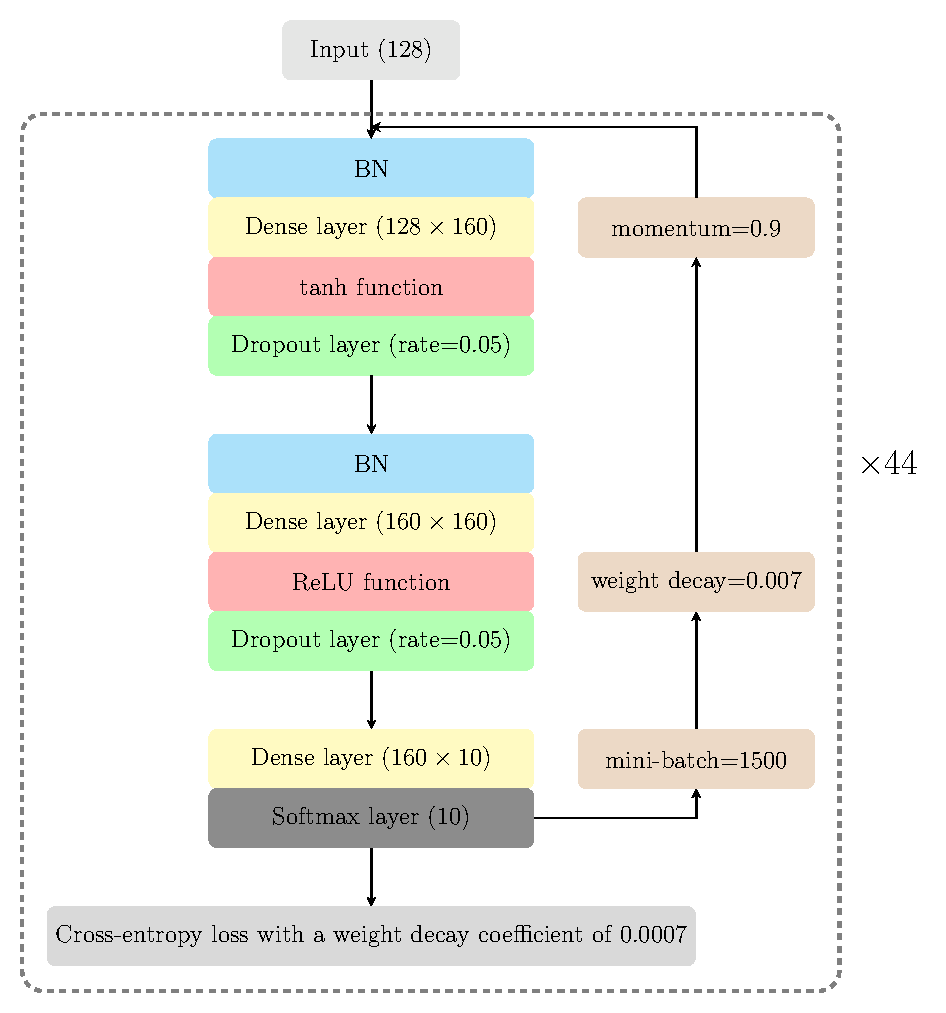
\includegraphics[scale=0.7]{NN.pdf}
    \caption{A diagram illustrates the architecture of our benchmark neural network model. The weights of the densely connected layers are initialised by a uniform distribution proposed by \citet{pmlr-v9-glorot10a}.}
    \label{fig:nn}
\end{figure}
For each of the three activation layers~$i=1,2,3$, this report uses $\vec t_i=(t_{i1},t_{i2},\ldots)$ to denote the the inputs of the $i$th densely connected layer
\footnote{We use $(\ )$ to denote column vectors, and $[\ ]$ to denote row vectors.}
, and uses $\vec z_i=(z_{i1},z_{i2},\ldots)$ to denote the outputs of the $i$th activation layer. 
We apply batch normalisation (BN) to normalise the input data~from $\vec t_1$ to~$\tilde{\vec t}_1$. This is followed by a nonlinear activation function. After the first hidden layer, our neural network applies a dropout layer, followed by an additional BN to the normalised outputs. 
We then apply an densely connected layer with a ReLU activation function, an additional dropout layer. The neural network finishes with a Softmax activation layer. 

\subsection{Cross validation score and early stopping prevents overfit\label{sec:early}}
We partition our dataset into $50,000$ training samples and $10,000$ test samples. For each epoch, we first train our model using the training samples and then compute the cross validation (CV) accuracy using the test samples. After $200$ epoch, we find the number of epoch~\texttt{n\_iter} corresponding to the maximum CV accuracy as our early stopping point. Using all the $60,000$ samples, we then train our model again  \texttt{n\_iter} epoches to obtain our final neural network model.

\subsection{Cross-entropy with weight decay improves the model robustness}
Define~$\vec y_k:=(y_{1k},y_{2k},\ldots,y_{10k})$ as the one hot encoding of the training label for the $k$th sample and $\vec p_k:=(p_{1k},p_{2k},\ldots,p_{10k})$ as the corresponding predicted probabilities. To train the neural network, we apply the cross-entropy loss 
\begin{equation}
  {L(\vec p|\vec y)=-\sum_{k}\sum _{j=1}^{10} y_{jk}\log p_{jk}}.  \label{eq:loss}
\end{equation}

Although the structure of our neural network is relative simple, it still has too many parameters. For example, if we set the number of hidden nodes in each hidden layer to be 160, then the number of parameters to estimate in the weights~$W_1,W_2$ and $W_3$ is $128*160+160*160+160*10=47,680$. The total number of parameters including biases~$b_i$ and BN parameters~$\gamma_i$ and~$\beta_i$ is more than $47,680$. As we only have $50,000$ training samples, allowing entries of the weights~$W_i$ to be arbitrary real number overfits the dataset. To encounter this ill-proposed problem, we penalise the complexity of our model by a $L2$ regularisation term as proposed by \citet{doi:10.1080/00401706.1970.10488634}
\begin{equation}
  {L=-\sum_k\sum _{j=1}^{10} y_{jk}\log p_{jk}}+\lambda\sum _{i=1}^3\left|W_i\right|^2,  \label{eq:loss_reg}
\end{equation}
where hyperparameter~$\lambda$ is a positive real number.
In comparison with loss function~\eqref{eq:loss}, the regularised loss function~\eqref{eq:loss_reg} penalises the model to have large weight matrices~$W_i$ and hence reduces the model complexity.

The reason to choose cross-entropy loss lies in its derivative. Taking the derivative of loss function~\eqref{eq:loss_reg}
\begin{equation*}
  \frac{\partial L}{\partial z_{3j}}=\sum_k p_{jk}-y_{jk}+\lambda\frac{\partial }{\partial z_{3j}}\sum _{i=1}^3\left|W_i\right|^2.  
\end{equation*}
This derivative function has a key property that many other loss functions like mean square loss do not have---the larger the errors~$\sum_k p_{jk}-y_{jk}$ is, the faster all the neurons will learn.

\subsection{Xavier initialisation speeds up convergence\label{sec:xav}}
We initialise the weight matrix~$W_i$ for $i=1,2,3$ using Monte Carlo method from a uniform distribution bounded by $\pm \sqrt{6/\left[\dim(z_i)+\dim(t_i)\right]}$ as suggest by \citet{pmlr-v9-glorot10a}. We use $0$s as the initial condition for bias vector~$\vec b$. As a result, the weight decay term helps to prevent the neural network from overfitting.

We also have experimented to use the normal distribution initialisation suggested by \citet{pmlr-v9-glorot10a}, but it is outperformed in accuracy and speed. So, it is not discussed here.

Xavier initialisation makes sure the initialised weights and biases are not too far away from the optimal weights and biases \citep{pmlr-v9-glorot10a}. This is essential because a poorly initialised optimisation problem usually either ends up with a solution that is far away from global optimum, or even diverges.

\subsection{BN prevents internal covariance shift}
We normalise the inputs~$t_{ij}$ for layers~$i=1,2$. When training using mini-batch~$B$ as defined in Section~\ref{sec:minibatch}, we use $\mu_B^{(j)}$ and $\sigma_B^{(j)^2}$ to denote the sample mean and sample variance for the mini-batch~$B$. Here, index~$j$ denotes one dimension of the input data. Moreover, we define $\gamma_{ij}$ and $\beta_{ij}$ ($i=1,2$) as real parameters to be learnt by backward proporgation. The BN layer iteratively normalise each dimensions~$j$ of the input batch as
\begin{equation}
     {\tilde {t}}_{ij}=\gamma_{ij}\frac {{t}_{ij}-\mu _{B}^{(j)}}{\sqrt {\sigma _{B}^{(j)^{2}}+10^{-8} }}+\beta_{ij} \text{ where } i=1,2.
\end{equation}
When predicting test labels, we use the training means~$\frac{1}{\left|B\right|}\sum_B \mu_B^{(j)}$ and training  variances~$\frac{1}{\left|B\right|}\sum_B \frac{\left|B\right|}{\left|B\right|-1}\sigma_B^{(j)^2}$ to normalise the test inputs.
Our neural network applies this BN layer to prevents internal covariance shift \citep{pmlr-v37-ioffe15}. Later on, \citet{NIPS20187515} find that BN makes the optimisation landscape considerably smoother.

\subsection{Dropout performs model averaging}
We apply dropout to the inputs of the 2nd and 3rd densely connected layers~$\vec t_2$ and $\vec t_3$, as proposed by \citet{dropout}. 
When training our neural network, the dropout layer randomly ignores neurons in vectors~$\vec t_2$ and $\vec t_3$ with a given probability hyperparameter~$p$. 
When predicting labels for CV samples and testing samples, we multiply weights~$W_i$ where layer index~$i=2,3$ by hyperparameter~$p$. This dropout layer is equivalent to model averaging, and forces our neural network to learn a more robust set of parameters that are useful in conjunction with many distinct random subsets of the neurons \citep{DBLP:journals/corr/abs-1207-0580}.

\subsection{Activation functions map input to desired output range}
Our neural network model has three densely connected layers. These three layers respectively implements a nonlinear activation function, a ReLU activation function, and a Softmax activation function.
\subsubsection{Nonlinear activation\label{sec:nonl}}
The first densely connected layer is chosen to be either of a hyperbolic function 
\begin{equation}
 \vec z_1(\tilde{\vec  t}_1)=\tanh(W_1\tilde{\vec  t}_1+\vec b_1) \label{eq:tanh}
\end{equation}
or a sigmoid function 
\begin{equation}
  \vec z_1 (\tilde{\vec  t})_1 =  {\vec 1}\left/\left[\vec 1 + \exp\left(W_1\tilde{\vec  t}_1+\vec b_1 \right)\right]\right.  \label{eq:sig}
\end{equation}
where matrix~$W_1$ is a $160\times128$ weighting matrix and vector~$\vec b$ is an $160$-dimensional bias vector. 
Here, the division~$/$ is an elementwise operator.
This layer provides non-linearity to our neural network.
\subsubsection{ReLU activation function}
The second densely connected layer is the piece-wise linear function named as ReLU
\begin{equation*}
   \vec z_2(\tilde{\vec  t}_2)=\max(0,W_2\tilde{\vec  t}_2+\vec b_2).
\end{equation*} 
ReLU guarantees the output of the layer is sparse. The nonlinear activation functions~\eqref{eq:tanh} and~\eqref{eq:sig} do not have this property. 
The sparseness makes the neural network more computationally efficient \citep{NIPS20145267}.
\subsubsection{Softmax activation function}
The Softmax activation functions takes a vector of real numbers as the input, and convert it into a categorical distribution as the output. Define matrix~$\mathbf 1$ to be a $10\times 10$ matrix of ones so that multiplying by matrix~$\mathbf 1$ is equivalent to summing up all rows. The activation function is the probability mass function of this categorical distribution
\begin{equation}
     \vec z_{3}(\vec t_3)={\exp(W_3 \vec t_{3}+\vec b)}\left/\left[{\mathbf 1\exp{(W_3 \vec t_{3}+\vec b)}}\right]\right.,
\end{equation}
which sums up to one. We assign the index of probability vector~$\vec z_{3}(\vec t_3)$ corresponding to the largest probability as the classification result for the corresponding sample.

\subsection{Stochastic gradient descent finds the optimal weights}
We use gradient descent with mini-batch and momentum to iteratively find optimise our model.
\subsubsection{Mini-batch improves the speed of computation \label{sec:minibatch}}
Traditional batch gradient descent uses all samples to estimate the gradient of the loss function. Estimating such a gradient using this way may be a very computationally expensive procedure. Alternatively, stochastic gradient descent uses only one sample to estimate the gradient. Although it economises the computational cost, the non-smooth nature makes the convergent much slower. 
We applied mini-batch as a compromise between the true gradient descent and the stochastic gradient descent methods. 
Instead of using either all samples or only using one sample to estimate the gradient, we use $1,000$ training samples (i.e. a ``mini-batch''~$B$) at each step. 
In comparison with stochastic gradient descent, mini-batch naturally takes advantage of the vectorisation nature of the \texttt{numpy} library and converges much faster \citep{DBLP:journals/corr/GoyalDGNWKTJH17}.

\subsubsection{Momentum accelerates rate of convergence}
We use~$\eta$ to denote the learning rate, $\alpha$ to denote the momentum coefficient and $\nabla$ to denote the gradient operator. In the $s$th iteration, assume that the first order Taylor expansion of the loss function~\eqref{eq:loss_reg} informs to update the weight matrix~$W_i$ as $W_i^{(s+1)}:=W_i^{(s)}-\eta\nabla L(W_i^{(s)})$, the gradient descent update with momentum proposed by \citet{rumelhart1986learning} is
\begin{equation*}
    \Delta W_i^{(s+1)}=\alpha \Delta W_i^{(s)}-\eta \nabla L(W_i^{(s)})\text{ and } W_i^{(s+1)}=W_i^{(s)}+\Delta W_i^{(s+1)}.
\end{equation*}
To initialise this update, we set $\Delta W_i^{(0)}:=0$. This autoregressive update proposal smooths the wiggliness caused by stochastic gradient descent \citep{rumelhart1986learning}, and hence significantly accelerates the rate of convergence.

%\subsubsection{todo: adam}

\section{Experiments}\label{chapter4}

\subsection{Dataset}
We illustrate our two \textsc{nmf} algorithms on two real-world face image datasets: \texttt{ORL} and \texttt{CroppedYaleB} (\citet{belhumeur1997eigenfaces}).
Both \texttt{ORL} and \texttt{CroppedYale} datasets contain multiple images of distinct subjects with various facial expression, lighting condition, and facial details.
Images in ORL are cropped and resized to $92 \times 112$ pixels. We further rescale it to $30 \times 37$ pixels. Similarly, we reduce the size of images in \texttt{CroppedYale} to $42 \times 48$ pixels.
For each dataset, we flatten the image matrix into a vector and append them together to get a matrix $V$ with shape $d\times n$ where integer~$d$ is the number of pixels in one image and integer~$n$ is the number of images. In each epoch, we use 90\% of data.

\subsection{Noise}
We implement three kinds of noises including Gaussian noise, Poisson noise and Salt \& Pepper noise.
\subsubsection{Gaussian Noise}\label{sec:gau}
We design the Gaussian noise by a normal distribution with a mean of $0$ and a standard deviation of $80$ (Algorithm~\ref{gau}). The \texttt{ORL} dataset has a global pixel mean of $40$ and the \texttt{CroppedYale} dataset has that of $70$. Hence the designed Gaussian noise contaminates the images significantly. We choose the standard deviation to be $80$ so that our Gaussian noise is less likely to coincident with the designed Poisson noise. To satisfy the nonnegative constant, negative value in the contaminated image is set to zero.
\begin{lstlisting}[caption= Gaussian Noise Design, label=gau]
def normal(subVhat):
    """Design a Gaussian noise."""
    V_noise = np.random.normal(0, 80, subVhat.shape) #* np.sqrt(subVhat)
    V = subVhat + V_noise
    V[V < 0] = 0
    return V, V_noise
\end{lstlisting}


\subsubsection{Poisson Noise}\label{sec:poi}
The Poisson noise is not additive and has no hyperparameters to be set. Unlike Gaussian noise, contaminated images are drawn directly from Poisson distributions with parameters set to be pixel values. Then, the Poisson noise is calculated from the difference between the contaminated image and the original image, as discussed in Section~\ref{chapter2} and demonstrated in Algorithm~\ref{poi}.
\begin{lstlisting}[caption= Poisson Noise Design, label=poi]
def possion(subVhat):
    """Design a Possion noise."""
    V = np.random.poisson(subVhat)
    V_noise = V-subVhat
    return V, V_noise
\end{lstlisting}


\subsubsection{Salt \& Pepper Noise}\label{sec:sal}
% JOYCE please add here
Salt \& Pepper noise (Algorithm~\ref{salt}) is added by drawing random integers from the discrete uniform distribution of the interval $[0, 255)$ . We find the bright places in generated image and replace pixel values in the same place of the original image with the brightest value. Similarly, we also find the dark pixels in the  images and replace pixel values in the same place of original image with the  darkest pixel value. In this case, we set the pixels whose values are greater than or equal to 230 as bright pixels and pixels whose value being less than or equal to 20 as dark pixels.
\begin{lstlisting}[caption= Salt and Pepper Noise Design, label=salt]
def salt_and_pepper(subVhat):
"""Design a salt and pepper noise where make some pixel value zeros."""
  V_noise = np.random.randint(low=0, high=255, size=subVhat.shape, dtype=int)
  V = subVhat.copy()
  V[V_noise <= 20] = 0
  V[V_noise >= 230] = 255
  return V, V_noise
\end{lstlisting}

\subsection{Experiment Setup}

We apply two algorithms (\textsc{nmf} and \textsc{klnmf}) with four categories of noises (no noise, Gaussian noise, Poisson noise and Salt \& Pepper noise), which results in eight combinations in each epoch. In each epoch, we randomly select 90\% of samples to train NMF algorithms and evaluate three metrics on reconstructed images. The training will terminate when the error reaches the minimum error, or the maximum iteration is reached. The minimum error and maximum iteration are hyperparameters which we learn from iterative experiments. Our code saves the learning errors versus the number of iterations so that we could draw the plot and observe the convergence of the learning process. We increase the number of epochs and calculate the average metrics and confidence intervals.


\subsection{Experiments Results}
\subsubsection{Two algorithms output similar reconstructed images}
Figure~\ref{noisesnmff} and~\ref{noisesklnmff} visualise the original image, designed noises, corrupted images and reconstructed images from left to right. From top to bottom, the four rows correspond to no noise, Gaussian noise discussed in Section~\ref{sec:gau}, Poisson noise discussed in Section~\ref{sec:poi} and Salt \& Paper noise discussed in Section~\ref{sec:sal}.
The first row of Figure~\ref{noisesnmff} and~\ref{noisesklnmff} show both algorithms reconstructed the original image well without artificial noise and with Poisson noise.
\begin{figure}
	\centering
	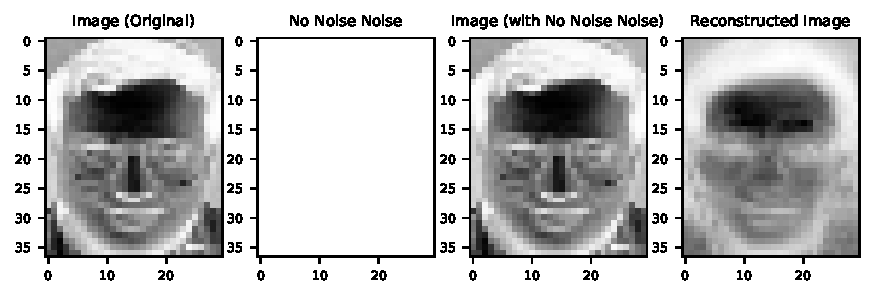
\includegraphics[scale=.9]{Result_Multiplication_Euclidean_No_Noise_Comparison}\\
	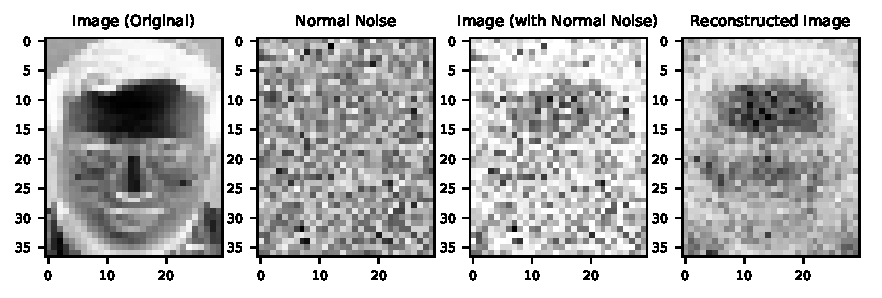
\includegraphics[scale=.9]{Result_Multiplication_Euclidean_Normal_Comparison}\\
	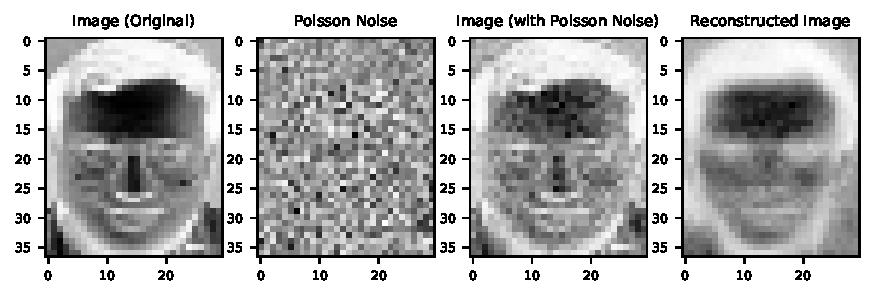
\includegraphics[scale=.9]{Result_Multiplication_Euclidean_Poisson_Comparison}\\
	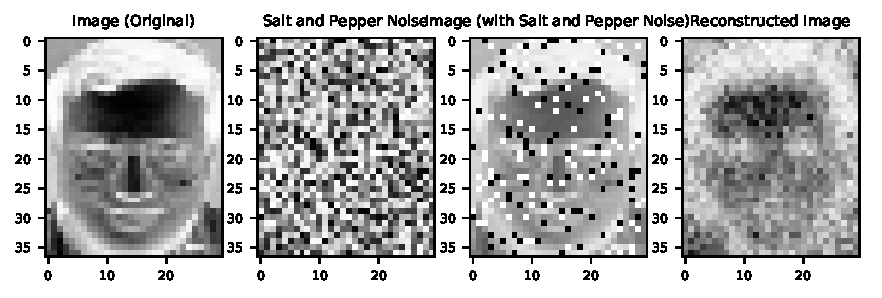
\includegraphics[scale=.9]{Result_Multiplication_Euclidean_Salt_and_Pepper_Comparison}
	\caption{The reconstructed image by \textsc{nmf}. The original images (Column~1) are combined with noises (Column~1) including Gaussian Noise with Variance~$80$ (Row~2), Poisson Noise (Row~3), and Salt \& Pepper Noise (Row~4). The corrupted images are shown in Column~3. The reconstructed images are shown in (Column~4). The reconstruction with no noise is shown in Row~1.}\label{noisesnmff}
\end{figure}
\begin{figure}
	\centering
	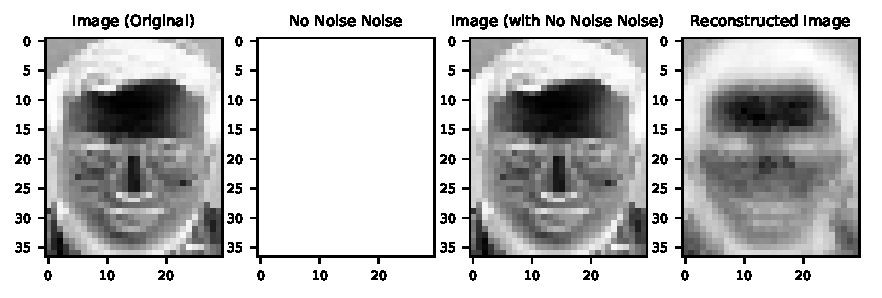
\includegraphics[scale=.9]{Result_Multiplication_KL_Divergence_No_Noise_Comparison}\\
	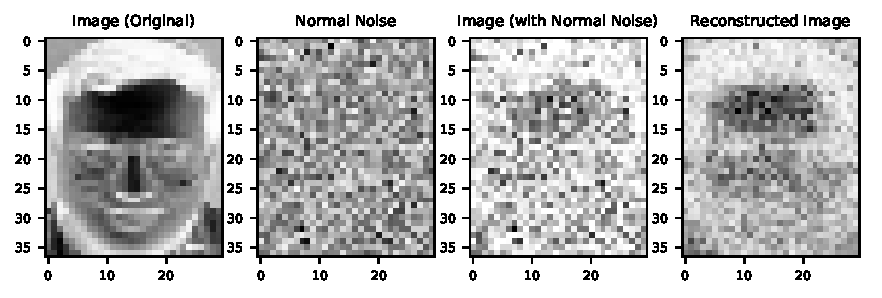
\includegraphics[scale=.9]{Result_Multiplication_KL_Divergence_Normal_Comparison}\\
	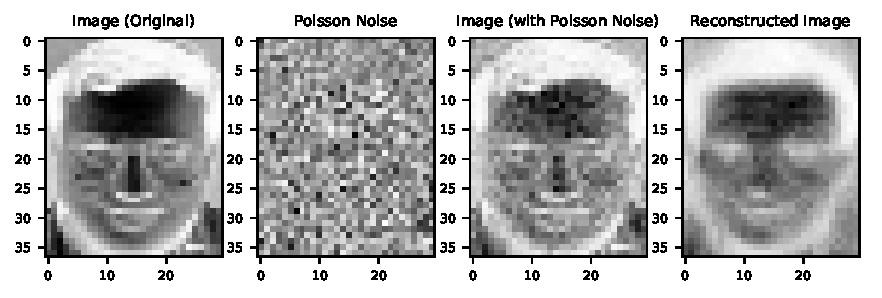
\includegraphics[scale=.9]{Result_Multiplication_KL_Divergence_Poisson_Comparison}\\
	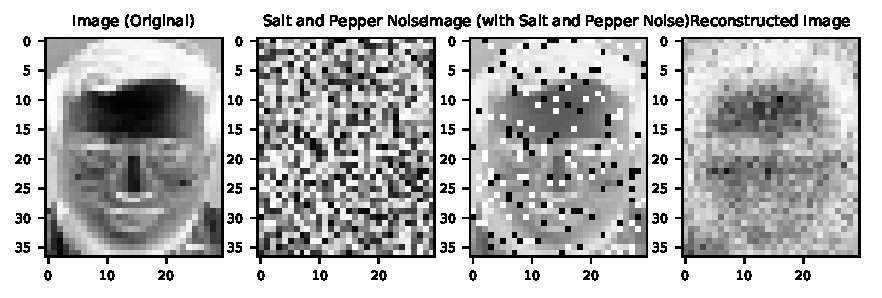
\includegraphics[scale=.9]{Result_Multiplication_KL_Divergence_Salt_and_Pepper_Comparison}
\caption{The reconstructed image by \textsc{klnmf}. The original images (Column~1) are combined with noises (Column~1) including Gaussian Noise with Variance~$80$ (Row~2), Poisson Noise (Row~3), and Salt \& Pepper Noise (Row~4). The corrupted images are shown in Column~3. The reconstructed images are shown in (Column~4). The reconstruction with no noise is shown in Row~1.}\label{noisesklnmff}
\end{figure}
However, when the noise is large (the second and last rows in Figure~\ref{noisesnmff} and~\ref{noisesklnmff}), the quality of reconstructed images looks marginally better than the contaminated images.
This result is consistent with \citet{guan2017truncated}, who assert that \textsc{nmf} may fail to handle extremely corrupted images when we violate the assumptions on the distributions of noise.
Moreover, the difference between images generated by \textsc{nmf} and \textsc{klnmf} are not visually significant.
Hence, we implement the statistical hypothesis test to compare of \textsc{rre}s of the two algorithms.

\subsubsection{Hypothesis test distinguishes the difference in RRE}
Substitute \href{https://raw.githubusercontent.com/JoyceXinyueWang/nmf_raw_data/master/raw_result_acc.csv}{\textsc{rre} results} (Figure~\ref{histo}) from $80$ Monte-Carlo simulations of the two algorithms into Kolmogorov-Smirnovs test~\eqref{teststatistic} gives test statistics~$D=1, 1 ,0.6625$ with no noise, Gaussian noise, and Poisson noise, for the \texttt{ORL} dataset. These three test statistics are all much greater than the critical value~$0.215$. Hence there are strong statistical evidences that the performance of \textsc{nmf} and \textsc{klnmf} are different in these three problems. For salt and Pepper noise, test statistic~$D=0.2125<0.215$, hence we fail to conclude that the two methods have different robustness against Salt and Pepper noise. Further, one tail Kolmogorov-Smirnov test concludes that \textsc{klnmf} performs better reconstructing the original image with no noise and is more robust Poisson noise. 
In contrast, \textsc{nmf} is more robust against Gaussian noise, even with only $500$ iterations ($1200$ for \textsc{klnmf}).
\begin{figure}
{\centering
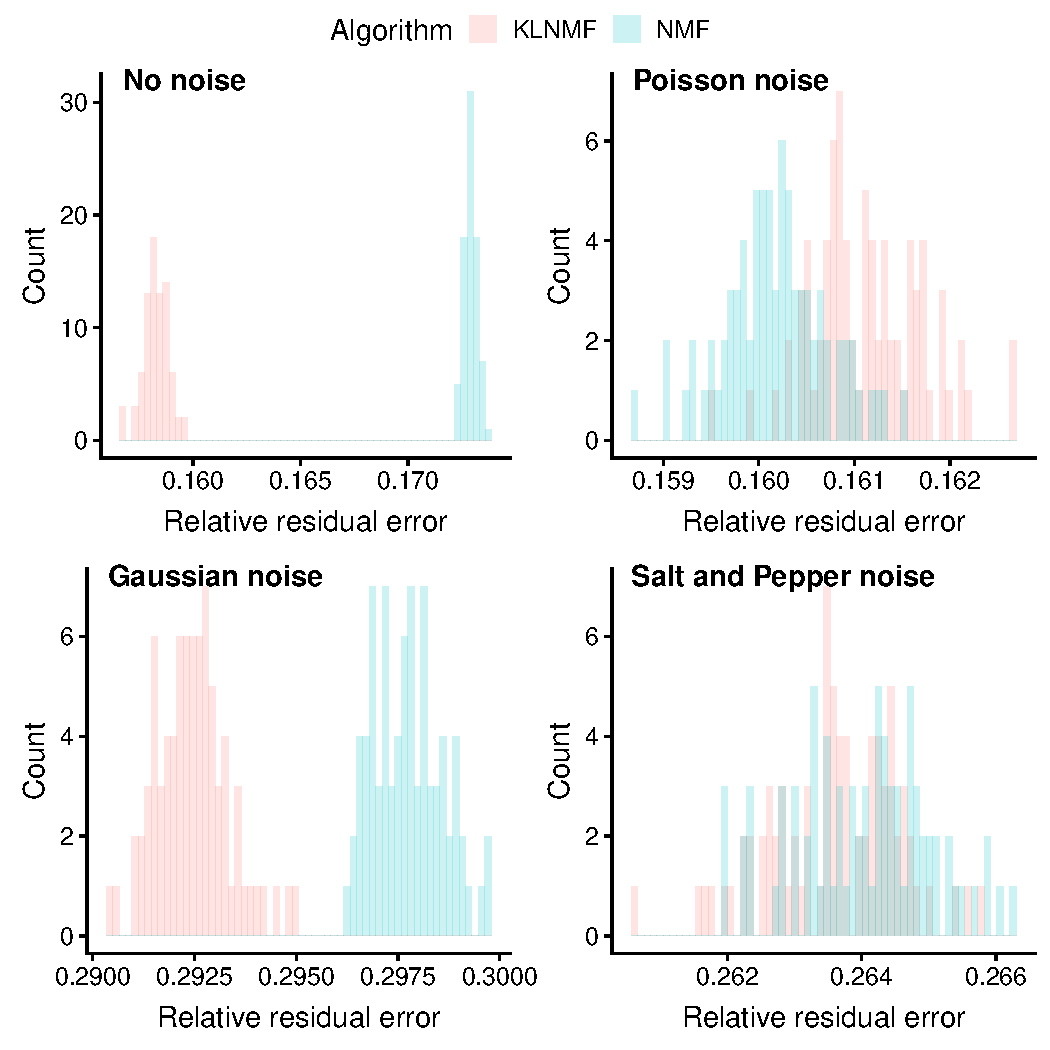
\includegraphics[scale=0.8]{histo}
\caption{Histogram of \textsc{rre} results from 80 Monte-Carlo simulations. Blue bars correspond to \textsc{nmf}, and the pink bars correspond to \textsc{klnmf}. The types of noise are labelled in the plot. The visualisation agrees with our statistical analysis.}
\label{histo}}
\end{figure}

Theoretical results discussed in Section~\ref{chapter2} suggest \textsc{nmf} is more robust against Gaussian noise whereas \textsc{klnmf} is more robust against Poisson noise. Our experimental results concluded from Kolmogorov-Smirnovs hypothesis tests agree with these theoretical results. Further, as both of the algorithms are not designed for Salt and Pepper noise, they have a similar performance against it.

These results can be observed by directly reading whether the confidence intervals overlap in Table~\ref{tab:ci}. Also, the statistical results agree with the visualisation in Figure~\ref{histo},~\ref{noisesnmff} and~\ref{noisesklnmff}. These results also agree with our intuition---although the differences in the robustness of the two algorithms are small, the even smaller variances in the \textsc{rre} results make them statistically different under Poisson and Gaussian noise (Figure~\ref{histo}).

With the \texttt{CroppedYale} dataset, the test results (Table~\ref{tb:yale}) agree with those of the \texttt{ORL} data as well as theories in Section~\ref{chapter2}: 1. against Poisson noise, \textsc{klnmf} with update rule~\eqref{eq:klnmf} has a lower \textsc{rre}; 2. against Gaussian noise, \textsc{nmf} with update rule~\eqref{eq:nmf} has a lower \textsc{rre}; 3. \textsc{klnmf} has a lower \textsc{rre} for images with no artificial noise. However, using \texttt{CroppedYale} dataset, the \textsc{nmf} algorithm performs much better against Salt \& Pepper noise. This might be a result of the \textsc{nmf}'s much faster convergence rate for large dataset, that is, the performance of \textsc{klnmf} might be significantly better with more iterations when processing \texttt{CroppedYale}. We did not perform more iterations for \textsc{klnmf} due to running time constraint.
%results from hypothesis tests show that \textsc{nmf} performs uniformly better than \textsc{klnmf}, suggesting more iterations are required on \textsc{klnmf} to compare these two algorithms fairly. We fail to do so because the dataset is much larger than \texttt{ORL} and our multiplicative update rules, especially for \textsc{klnmf} converge too slow.

\subsubsection{ACC and NMI results}
In terms of \textsc{acc} and \textsc{nmi}, the differences between \textsc{nmf} and \textsc{klnmf} under Gaussian noise and Salt \& Pepper noise are trivial given their overlapped confidence intervals. Under Possion noise, however, \textsc{klnmf} is superior than \textsc{nmf} for both measurements. 


\begin{table}
\caption{Average of evaluations metrics over $80$ Monte-Carlo simulations using the \texttt{ORL} dataset. The 95\% confidence intervals are calculated using bootstrap.}
\hspace{-1cm}{\small
\label{tab:ci}\begin{tabular}{l|lll}
 \hline
\texttt{ORL} dataset & \textsc{rre} & \textsc{acc} & \textsc{nmi}\tabularnewline
 \hline
\textsc{nmf} no noise & 0.1583 (0.1581, 0.1584) & 0.7364 (0.731, 0.742) & 0.8536 (0.8506, 0.8567)\tabularnewline

\textsc{nmf} Gaussian noise & 0.2925 (0.2922, 0.2927) & 0.447 (0.4423, 0.4521) & 0.6212 (0.6176, 0.6247)\tabularnewline

\textsc{nmf} Poisson noise & 0.1611 (0.161, 0.1613) & 0.7313 (0.7262, 0.7367) & 0.8493 (0.8456, 0.8527)\tabularnewline

\textsc{nmf} Salt and Pepper noise & 0.2636 (0.2634, 0.2638) & 0.5094 (0.504, 0.5151) & 0.6721 (0.6679, 0.6764)\tabularnewline

\textsc{klnmf} no noise & 0.1729 (0.1728, 0.173) & 0.7406 (0.7352, 0.7458) & 0.8599 (0.8568, 0.8632)\tabularnewline

\textsc{klnmf} Gaussian noise & 0.2977 (0.2976, 0.2979) & 0.4538 (0.4483, 0.4595) & 0.6209 (0.6165, 0.6255)\tabularnewline

\textsc{klnmf} Poisson noise & 0.1602 (0.1601, 0.1603) & 0.7417 (0.7365, 0.7472) & 0.8573 (0.8542, 0.8602)\tabularnewline

\textsc{klnmf} Salt and Pepper noise & 0.264 (0.2638, 0.2643) & 0.5089 (0.5038, 0.5139) & 0.6734 (0.6694, 0.6779)\tabularnewline
 \hline
\end{tabular}}
\end{table}

%In terms of the \texttt{CroppedYale} dataset, results from hypothesis tests show that \textsc{nmf} performs uniformly better than \textsc{klnmf}, suggesting more iterations are required on \textsc{klnmf} to compare these two algorithms fairly. We fail to do so because the dataset is much larger than \texttt{ORL} and our multiplicative update rules, especially for \textsc{klnmf} converge too slow. Note that accuracy of \texttt{CroppedYale} is small overall. This is because we rescale the images in \texttt{CroppedYale} by factor 4 whereas we only rescale the images in  \texttt{ORL} by factor 3. Besides, there are more cropped images in  \texttt{CroppedYale} and there are more labels in  \texttt{CroppedYale}. All of them contribute to the low accuracy.

\begin{table}
\caption{Average of evaluations metrics over 10 Monte-Carlo simulations using \texttt{CroppedYale} dataset.}
\centering
\hspace{-1cm}{
\label{tb:yale}\begin{tabular}{l|lll}
 \hline
\texttt{CroppedYale} dataset & \textsc{rre} & \textsc{acc} & \textsc{nmi}\tabularnewline
 \hline
\textsc{nmf} no noise & 0.2022 & 0.2377 & 0.3204\tabularnewline

\textsc{nmf} Gaussian noise & 0.3114 & 0.2116 & 0.2777\tabularnewline

\textsc{nmf} Poisson noise & 0.2023 & 0.2442 & 0.3241\tabularnewline

\textsc{nmf} Salt and Pepper noise & 0.2748 & 0.2133 & 0.2902 \tabularnewline

\textsc{klnmf} no noise & 0.2062 & 0.2434 & 0.3191 \tabularnewline

\textsc{klnmf} Gaussian noise & 0.3106 & 0.2112 & 0.2845 \tabularnewline

\textsc{klnmf} Poisson noise & 0.2065 & 0.2377 & 0.3104\tabularnewline

\textsc{klnmf} Salt and Pepper noise & 0.3164 & 0.1634 &0.2332 \tabularnewline
 \hline
\end{tabular}}
\end{table}
\subsection{Personal Reflection}
The implementation of this project was challenging and rewarding. We overcome many problems that are not taught in class by research. For instance, we learnt to use multi-start algorithm with parallel computing to overcome the problem that ~\textsc{klnmf} always gets stuck into local optimal. 
In addition, we learnt that although one algorithm performs better than another one theoratically, it might require more running time. In real implementation, we need to consider the running time versus performance trade-off. For example, the ~\textsc{klnmf}  multi-start parallel computing has overall better performance than ~\textsc{nmf}; however, it has slow convergence rate and multi-start parallel computing will cost more than than non-multi-start ~\textsc{klnmf} algorithm, especially when training \texttt{CroppedYale} dataset .
Moreover, we critically considered what truly defines a `good' algorithm. Although theoretically privileged algorithms may be good for handling difficult tasks, they tend to be time-consuming and not easy to implement. For example, through literature review, we found some algorithms such as Truncated Cauchy \textsc{nmf} \citet{guan2017truncated} that are excellent for contaminated data but too difficult for us to implement. Hence, in real-world practice, simpler and faster algorithm may be more widely used than advanced algorithms. 
Lastly, we observed many interesting results during the experiment. For instance, we found that the \textsc{rre}s of \textsc{klnmf} with Poisson noise is superior to that with no noise in \texttt{ORL} dataset. %One hypothesis is that added Poisson noise neutralised the noise from the original image. Another hypothesis is that 
This may result from the noise assumptions made by these two algorithms. 


\section{Conclusion}
In conclusion, our numerical simulation supports the published results on various state-of-the-arts modules. We find BN is the most significant module to improve CV accuracy and predictive capability. In terms speed, mini-batch training is the most important module follow by the momentum method. However, the size of the batch as well as the momentum coefficients need to be carefully tuned. Also, simulation results shows that dropout is useful for large neural networks where the number of parameters is large comparing with the number of samples. We use shell script to train neural network models with different hyperparameters in a parallel setting. Parallel computing fully utilises our computing resources and double the speed to train ten neural network models.

In recent years, \textsc{nvidia} released their \href{https://developer.nvidia.com/cuda-zone}{\texttt{Cuda}} package which parallelises matrix multiplications using \textsc{gpu}. Large and iterative matrix multiplications is the most computational intensive part when training neural network, This package improves the speed of matrix multiplication by a factor of $>200$. As a computationally expensive procedure, a natural extension of this project is to implement \href{https://developer.nvidia.com/cuda-zone}{\texttt{Cuda}} to speed up the training speed of our neural network. \citet{5452452} shows that GPU performs 2 to 24 times faster than on the CPU on accelerating training and classification of arbitrary Convolutional Neural Networks (CNNs).


%\appendix
\section{Appendix}


\titleformat{\section}
    {\normalsize\bfseries\centering}{\thesection}{5pt}{\normalsize}
\bibliography{research}

\end{document}
